% !TEX encoding = UTF-8 Unicode 
%
% Use:
% magister / inzynier - for master thesis or engineering thesis
% druk / archiwum - for print version or archive version
% en - to translate template into english
% examples:
%\documentclass[inzynier,druk,en] - master thesis, print version, english
%\documentclass[magister,druk,en]{dyplom}
%\documentclass[magister,druk]{dyplom}

\PassOptionsToPackage{table}{xcolor}

\documentclass[inzynier,druk]{dyplom}

\newcommand{\nl}{\\ \hline}
\newcommand{\dnl}{\\ \hline \hline}

% CUSTOM HERE
% kwestia do rozważenia
% \usepackage[draft,nosingleletter]{impnattypo}

% END CUSTOM HERE

\usepackage[utf8]{inputenc}
\usepackage{hyperref}

% Maximum section's depth.
\setcounter{secnumdepth}{4}

% Listings settings
\setminted{breaklines,
frame=lines,
framesep=3mm,          
baselinestretch=1.1,   
fontsize=\small,       
% linenos              % line numbering
}

\usepackage{lipsum}

% \faculty{Faculty of \dots}
\fieldofstudy{Inżynieria Systemów (INS)}
\author{Przemysław Grzegorz Barcicki}
\title{Moduł samouczący do systemu automatyki domowej}
\supervisor{dr. inż. Patryk Schauer}
% \specialisation{Inżynieria Danych (IND)}
\keywords{automatyzacja domowa, uczenie maszynowe, smart-home, python, tensorflow}

\begin{document}

\maketitle

\abstract{
Niniejsza praca ma na celu rozwiązanie problemu tworzenia złożonych reguł automatyzacji w systemach \textit{smart-home} poprzez wykorzystanie uczenia maszynowego i metod data-miningu. Moduł jest skierowany do osób, które chcą wypróbować możliwości jakie daje automatyzacja domu, bez konieczności tworzenia reguł dla każdego działania w ich codziennym życiu. Wyodrębniając epizody interakcji użytkownika z zapisanej historii HomeAssistant, moduł tworzy dane dla sieci neuronowych, które próbują przewidzieć następne działanie użytkownika i w przypadku wspólnego zamiaru, wykonuje je. Moduł ma być jak najbardziej rozszerzalny poprzez wdrożenie zorientowanego na obiekty modelu oraz wykorzystanie wolnego i otwartego oprogramowania.
}{
This work aims to solve the issue of creating complex automation rules in smart home systems by using machine learning and data mining. The module is addressed to people who are eager to try out the prospects made possible by home automation without the hassle of creating rules for every action in their day-to-day lives. By extracting the episodes of user interaction from HomeAssistant logs, it creates data for neural networks that try to predict the user’s next action and, in cases of common intent, execute them. Module aims to be as extendable as possible by implementing object-oriented design and by using free and open source software.
}

\tableofcontents

% !TEX encoding = UTF-8 Unicode 

\chapter{Wstęp}

\section{Wprowadzenie do problematyki}

Automatyzacja to określenie na metody mające na celu ograniczenie ludzkiej interakcji do minimum w różnych procesach. Stosuje się ją w wielu dziedzinach począwszy od przemysłu, kończąc na procesach informatycznych. Pewnym obszarem zyskującym w ostatnim czasie dużo zainteresowania jest pojęcie inteligentnego domu (smart-home). Automatyka domowa to konkretne określenie na zastosowanie automatyzacji wśród urządzeń smart-home skupiających się na obszarze zastosowań gospodarstwa domowego. Celem takiego zastosowania jest kontrola pracy urządzeń znajdujących się w domu do osiągnięcia konkretnego ich stanu w sposób minimalizujący ludzką interakcję. W praktyce takie systemy to bardzo dobre rozwiązanie które niesie ze sobą wiele zalet i uproszczeń w codziennym życiu \cite{szablowski2019projektowanie}.
% https://automatykab2b.pl/temat-miesiaca/39129-automatyka-budynkowa-czesc-1?show=1

Reguła w automatyce, czasem nazywana zasadą, to w dokładny sposób określenie jakie akcje muszą zostać wykonane pod warunkiem pewnego stanu systemu. Warunkiem początkowym może być każdy stan, zmiana stanu dowolnego urządzania lub całkowicie zewnętrzny bodziec. W przypadku takiej automatyzacji często też korzysta się z kombinacyjnego połączenia wielu źródeł i informacji w celu stworzenia stanu początkowego, który jeśli wystąpi, jest przesłanką do wysłania przez system zarządzający urządzeniami polecenia do wykonania pojedynczej lub ciągu akcji. Każde dostępne na rynku dedykowane oprogramowanie obsługujące automatykę domową dostarcza różne narzędzia do szybkiego i intuicyjnego sporządzania takich zasad, ale także dostarcza sposoby na komunikację z tymi urządzeniami. Dostepny jest zatem pełny system, który agreguje wiele pomniejszych mechanizmów, protokołów i sposobów wymiany danych w celu monitorowania i sterowania urządzeniami w ramach np. lokalnej sieci.

\section{Opis problemu}

Mimo tego, że analiza i projektowanie systemów inteligentnej automatyki domów zaczęła się kilka dekad temu, istnieje wiele nierozwiązanych problemów, które muszą zostać rozwiązane, aby autonomiczna forma stała się popularna. Ograniczeniami są nieprawidłowe algorytmy oraz niskie celności wynikowe \cite{episode_discovery_2}.

Mimo wygody w użytkowaniu i łatwości w sporządzaniu zasad automatyki domowej pojawiają się pewne trudności. Jednym z nich jest problem ze zmiennością ludzkich nawyków. Sporządzenie zasad sprawia, że dane czynności zostaną wykonywane wtedy i tylko wtedy gdy zostanie spełniony pewien konkretny stan określony przez użytkownika podczas sporządzania danej reguły. Z logicznego punktu widzenia jest to odpowiednia reakcja systemu, natomiast z tego praktycznego już nie, ponieważ dana reguła może zostać wykonana mimo tego, że w pewnych specyficznych okolicznościach użytkownik nie zechce aby się wykonała. Dodaje to pewien wymóg dalszego komplikowania danej zasady poprzez dodatkowe warunki w systemie lub ciągłe jej edytowanie aby odpowiadała naszym zmiennym nawykom.

Bez względu na to, jakie narzędzia dostarcza nam dany system, sporządzanie dużej liczby skomplikowanych reguł może być problematyczne. Same środowiska zarządzania takimi systemami mimo wspierania tworzenia na tyle skomplikowanych zasad mogą nie być do tego przystosowane. Często zdarza się, że system automatyki udostępnia dodatkowe, jako wtyczki lub dodatki, moduły do tworzenia reguł za pomocą interpretowanych języków programowania \cite{appdaemon:main}, \cite{domoticz:scripts}, \cite{openhab:scripts}. Tworzy to natomiast zestaw innych problemów, gdzie użytkownik chcący stworzyć takie reguły, musi w przynajmniej podstawowy sposób znać języki programowania, a ponadto mieć wiedzę w jaki sposób sporządzać te skrypty aby mogły być wykonywane przez oprogramowanie nadzorujące.


\section{Cel pracy}
Celem niniejszej pracy jest opracowanie modułu do systemu automatyki domowej (smart-home) wspierającego tworzenie reguł decyzyjnych w oparciu o mechanizmy uczące się zachowań użytkownika. Opracowane rozwiązanie powinno korzystać z wielu źródeł danych, czujników, stanu aktuatorów, źródeł zewnętrznych (np. prognoza pogody), stanu przełączników wyzwalanych przez użytkownika. Efektem działania modułu powinny być reguły możliwe do zastosowania w systemie automatyki lub bezpośrednio wywoływane w tym systemie akcje.

% to check: to co mam napisane w apd ma sie tu znaleźć
\section{Zakres pracy}
Zakres pracy obejmuje przegląd literatury w obszarze działania i budowy systemów wspomagania podejmowania decyzji opartych o uczenie maszynowe, a także przegląd tematyki związanej z działaniem i budową urządzeń Internetu Rzeczy z klasy smart-home. W zakresie również znajduje się projekt i implementacja prototypowego modułu samouczącego wraz z jego testami i integracją z istniejącym systemem autmatyki domowej.

% !TEX encoding = UTF-8 Unicode 

\chapter{Przegląd literatury}

% W tym rozdziale omówiono literaturę i istniejące rozwiązania problemu rozwiązywanego w dalszej części tej pracy. Pod uwage brano prace, które korzystają z klasycznych metod uczenia maszynowego oraz metod zawierających elementy sieci neuronowych. Analizie zostaną poddane użyte algorytmy jak i podejścia do osiągnięcia celu wspomagania decyzji automatyki domowej.

W tym rozdziale omówiono umiejscowienie tematu w literaturze. W pierwszej części opisano istniejące algorytmy i rozwiązania problemu. Pod uwagę brano te metody, które korzystają z klasycznych metod uczenia maszynowego oraz tych, które zawierają elementy sieci neuronowych. Analizie zostaną poddane użyte algorytmy jak i podejścia do osiągnięcia celu wspomagania decyzji automatyki domowej. W drugim etapie zawarte zostały opisy budowy i sposobów działania urządzeń Internetu Rzeczy.

\section{Algorytmy i rozwiązania}
\subsection{Systemy korzystające z algorytmów wykrywania epizodów}
\label{subsec:episode_discovery}
\textit{Episode discovery} (wykrywanie epizodów) to metoda data miningu (kopania danych) wykorzystująca istniejący ciąg występujących po sobie wydarzeń do wykrywania w nich powtarzalnych znaczących epizodów. Wśród epizodów można wyróżnić, tak zwane, epizody znaczące, które według zależnych od algorytmu charakterystyk, określają dany epizod jako często występujący.

Czesto można spotkać się pewną interpretacją ciągu zdarzeń w systemie gdzie każda występująca po sobie w pewnym oknie czasowym akcja jest reprezentowana jako odpowiedni znak ze zbioru wybranych możliwych zdarzeń. W przypadku opisu stanu systemu za pomocą reprezentacji znakowej, korzysta się z metodyki, gdzie duża litera oznacza przejście stanu danego urządzenia w załączone, a mała litera oznacza wyłączenie. W przykładowych ciągach zdarzeń, \verb|baDgb|, \verb|abD|, \verb|Dagb|. Można zauważyć, że zawsze po wystąpieniu wyłączenia urządzenia \verb|a|, następuje wyłączenie urządzenia \verb|b|. W rzeczywistości algorytmy są bardziej zaawansowane, ponieważ są w stanie wykryć epizody znaczące, które nie występują zawsze a w pewnym odsetku wszystkich wydarzeń i ponadto są w stanie operować na dużo dłuższych łańcuchach historycznych.

Wykorzystywanie algorytmów wykrywania epizodów na zapisanych już strumieniach wydarzeń pozwala na znalezienie pewnych nawyków i zależności z codziennego korzystania z domowych urządzeń. Znalezione i wyodrębnione epizody mogą zostać użyte z innymi algorytmami w celu podniesienia ich celności. Tak przetworzone dane wejściowe z dodatkowym użyciem innego algorytmu dają zdecydowanie lepsze wyniki niż w wypadku użycia samych sieci neuronowych bądź samego wykrywania epizodów \cite{episode_discovery_1}, \cite{episode_discovery_2}. 

% Smart Home Automation using IoT and Deep Learning 
% An Intelligent, Secure, and Smart Home Automation System
% Home Automation System Using IoT and Machine Learning Techniques
% Use of Prediction Algorithms in Smart Homes
% Smart Home Automation Using Machine Learning Algorithms
% A machine learning approach to predict the activity of smart home inhabitant
% Improving Home Automation by Discovering Regularly Occurring Device Usage Patterns

Ważnym elementem wykorzystania technik wykrywania epizodów jest prawidłowy wybór algorytmu (SPADE \cite{SPADE}, SPEED \cite{SPEED}, WINEPI \cite{WINEPI}, ...) jak i jego hiperparametrów, ponieważ inne wartości parametrów wybierających epizod znaczący mogą mocno wpływać na końcowy wynik \cite{episode_discovery_2}. O ile w przypadku algorytmu, nieprawidłowy wybór może ograniczać się do wydłużonego czasu poszukiwania epizodów, a co za tym idzie, większego zużycia zasobów przez system, tak w przypadku niewłaściwych parametrów, algorytm może proponować za dużo akcji i nawyków, które źle będą wpływały na końcowy wynik, co w końcu sprawi, że komfort korzystania z takiego systemu będzie niedostateczny.

Podejście wykrywania epizodów, jest metodą skupiającą się na pewnych ciągach zdarzeń, które nie biorą pod uwagę żadnych innych zewnętrznych parametrów. Sprawia to, że system uczy się ciągów wydarzeń bez względu na aktualny stan systemu, czyli na przykład porę dnia, temperaturę w pomieszczeniu, dzień tygodnia czy też pogodę. Połączenie klasycznych algorytmów \textit{episode discovery} z dodatkowymi algorytmami, które biorą pod uwagę inne parametry systemu, rozwiązuje ten problem, ale dodaje dużo skomplikowania w implementacji.

Korzystanie z metody dużych i małych liter do oznaczania wyłączeń i włączeń urządzeń tworzy dodatkowo pewne ograniczenia w postaci braku lub bardzo skomplikowanej obsługi urządzeń o niebinarnych stanach. O ile w przypadku urządzeń gdzie stanów jest kilka, jak na przykład systemy HVAC, można każdy z trybów pracy zinterpretować jako inną czynność, tak w przypadku urządzeń gdzie istnieje teoretycznie nieskończenie wiele stanów pośrednich, tak jak na przykład w ściemniaczach żarówkowych, nie jest możliwe reprezentowanie każdego z nich.

% \subsection{Systemy grafowe}
\subsection{Systemy korzystające z procesów Markowa}
Podczas modelowania zmian stanu systemu automatyki domowej można skorzystać z podejścia, gdzie próbujemy opisać ciąg zdarzeń za pomocą prawdopodobieństwa przejść między stanami. Bardzo pomocne w takiej strategii okazuje się korzystanie z modeli Markowa. Istnieje pewne rozszerzenie, które okazuje się bardziej pomocne w wypadku modelowania ludzkiej interakcji i zachowań z powodu uwzględnienia niezależnych i nieznanych przez model stanów, nazywane ukrytym modelem Markowa. Czyste podejście z prawdopodobieństwem odpowiada na pytanie, jaka jest szansa na wykonanie akcji \verb+A+ pod warunkiem tego, że poprzednio wykonana akcja to \verb+B+, dodatkowe ukryte informację pomagają w dokładniejszym określeniu przewidywanego stanu systemu.

Podobnie jak w przypadku wykrywania epizodów (\ref{subsec:episode_discovery}) do wytworzenia reprezentacji zmian systemu wykorzystywany jest literowy zapis, co sprawia, że te podejścia mają takie same ograniczenia. Jedna z prac \cite{markov_1}, próbuje rozwiązać problem związany z rzeczywistą (niebinarną) naturą pewnych stanów poprzez kwantyzację w konkretne stany. Konkretne wartości temperaturowe zamieniane są na arbitralny identyfikator wskazujący na daną temperaturę, co używane jest w modelu jako jeden z parametrów.

Podejście znalezione w \cite{markov_1}, próbuje rozwiązać, za pomocą autorskiej metody \textit{IHMM} (Improved Hidden Markov Models), problem powiązania pewnych konkretnych nawyków i ciągów wydarzeń z pewną temporalną zmienną, co sprawia, że system podpowiada konkretne akcje dokładniej o konkretnych porach dnia, lecz dalej nie rozwiązuje problemu rozpoznania np. dni tygodnia czy pogody.

Inna implementacja \cite{markov_2}, korzysta z innego, również autorskiego rozwinięcia modeli markowa \textit{TMM} (Task-based Markov Model). Metoda skupia się na zidentyfikowaniu wysokopoziomowych zadań, które to dalej są wykorzystywane do stworzenia pomniejszych modeli reprezentujących ciąg zdarzeń w konkretnym zadaniu. Zadania są identyfikowane na podstawie przerwy pomiędzy kolejnymi wydarzeniami oraz na podstawie dodatkowej informacji o lokalizacji danego urządzenia. Operacje wraz z informacjami o ilości, długości i położenia w przestrzeni używane są przez algorytm k-średnich do pogrupowania zadań i stworzenia zbioru konkretnych ciągów.

% TEORETYCZNE PODSTAWY ZASTOSOWAŃ UKRYTEGO MODELU MARKOWA DO ROZPOZNAWANIA WZORCÓW
% MavHome: An Agent-Based Smart Home
% Behavior prediction using an improved Hidden Markov Model to support people with disabilities in Smart Homes

% inne:
% MavHome: An Agent-Based Smart Home
% An Intelligent, Secure, and Smart Home Automation System
% Tu jest ładnie napisane dużo: Smart Home Automation using IoT and Deep Learning

\subsection{Sieci neuronowe}

% Automated Smart Home Controller Based on Adaptive Linear Neural Network 
% Smart Home Automation-Based Hand Gesture Recognition Using Feature Fusion and Recurrent Neural Network

Często spotyka się w parze z innym algorytmem sieci neuronowe, ponieważ są w stanie poprawić zdecydowanie celność predykcji niskim kosztem \cite{episode_discovery_1}. Istnieją pewne rozwiązania, gdzie sieci neuronowe są głównym sposobem na przeprowadzanie predykcji. Ich szerokie zastosowanie i wiele istniejących rozwiązań sprawia, że są w stanie występować na prawie każdej platformie obliczeniowej. Dodatkowo w ciągu ostatniej dekady widać było zdecydowany rozrost zastosowań i nowych rozwiązań korzystających w pewien sposób z głębokich sieci neuronowych.

Różne istniejące rozwiązania i modele głębokich sieci neuronowych daje duże pole do ich zastosowań. W przypadku pracy autorstwa S. Umamageswari \cite{neural_1}, zastosowano jedno z popularnych w ostatnim czasie rozwiązań \textit{LSTM} (long short-term memory). Rekurencyjne sieci neuronowe korzystające z warstw \textit{LSTM} są w stanie modelować pewne zależności w danych, występujące z dużym odstępem czasowym. Jest to dobre zastosowanie dla sieci wykorzystujących dużą ilość danych wejściowych zawierające informacje temporalne w odpowiedniej postaci. Takie modele matematyczne w procesie propagacji wstecznej błędu, są w stanie "nauczyć" się ciagu konkretnych zadań wykonywanych o konkretnych porach dnia, prezentując systemowi przykładowe historyczne wystąpienia tych zadań \cite{ksiazka_tf}.

Ciekawym podejściem okazuje się wykorzystanie konwolucyjnych sieci neuronowych w przypadku wprowadzania dodatkowych zmiennych do systemu \cite{conv_1}. System w celu określenia następnej akcji którą ma podjąć bierze pod uwagę wyraz twarzy użytkownika. Obraz twarzy, przekształcany jest przez sieci konwolucyjne do zestawu informacji mówiącym o samopoczuciu użytkownika.

\subsection{Podsumowanie i wnioski}
Biorąc pod uwagę przeprowadzoną analizę, widać, że wstępne przetwarzanie danych i odpowiednie ich spreparowanie jest bardzo kluczowe. Prawidłowa reprezentacja stanu w systemie jest bardzo ważna, ponieważ to na podstawie tego system będzie przeprowadzał swoje predykcje. W przypadku tradycyjnych algorytmów uczenia maszynowego widać ich zdecydowane ograniczenia, których rozwiązanie wymaga zdecydowanego komplikowania problemu poprzez wprowadzanie kwantyzowanych informacji czy zmiennych reprezentujących wartości temporalne. Metodą dającą największą elastyczność okazuje się wykorzystanie głębokich sieci neuronowych, ze względu na ich możliwość, przy wcześniejszym odpowiednim przekształceniu wejścia lub wyjścia, wprowadzania danych o różnych formatach, czy sterowania szerokim zakresem różnych urządzeń.

\section{Urządzenia IoT}

% A Survey based on Smart Homes System Using Internet-of-Things 
% Energy-Efficient System Design for IoT Devices
% An Overview of IoT Based Smart Homes
% A survey of Internet-of-Things: Future Vision, Architecture, Challenges and Services 
% What is a smart device? - a conceptualisation within the paradigm of the internet of things


Internet jest zbiorem technologii który bardzo zmienił sposób funkcjonowania ludzi. Wraz ze spadającym kosztem podłączenia urządzenia do internetu, znajdujemy coraz to nowsze zastosowania dla właśnie takich urządzeń. W ostatnich latach jesteśmy świadkami pewnej rewolucji w której ciągle podłączone do sieci urządzenia przenikają do naszego codziennego życia. Jako ludzie, posiłkujemy się tymi rzeczami w celu poprawy jakości i komfortu naszego istnienia \cite{iot_improves_lifes}. Aktualne czasy przyniosły ludzkości znaczący wzrost liczby zawsze podłączonych do internetu rzeczy w różnych obszarach, takich jak zdrowie, przemysł, transport czy rolnictwo. Jednym zastosowaniem, które cieszy się największą uwagą z urządzeń IoT (\textit{Internet-of-Things}), są takie, które sprawują swoje role w inteligentnych domach. W przypadku każdego z tych urządzeń w dowolnym zastosowaniu, można mówić o dwóch idących w parze elementach, którymi są osobno ,,rzecz'' i osobno ,,internet''.

\subsection{\textit{Rzecz}}
Kontekst rzeczy w domenie internetu rzeczy jest bardzo rozmyty, ze względu na swoją logiczną strukturę jak i fizyczne zastosowanie, co dalej tworzy podział na smart i nie-smart urządzenia. Literatura wyróżnia trzy elementy które definiują typ urządzenia. Są to: świadomość kontekstu, autonomia i łączność \cite{smart_dumb_devices}. Mowa tutaj o bardzo różnych systemach, które mogą agregować w jedność wiele czujników, wiele siłowników, procesorów i sposobów komunikacji. Do pierwszej z tych grup zaliczają się takie obiekty, które poza zbieraniem danych, są w stanie reagować na ich zmianę. Są to na przykład smart termostaty, które na podstawie temperatury zadanej i mierzonej decydują o odpowiedniej zmianie w swoim systemie. Mierzona temperatura może pochodzić z wprost z urządzenia lub też z innych urządzeń znajdujących się w środowisku. Do drugiej grupy, kontynuując poprzedni przykład, zaliczyć można urządzenia-satelity, które mają dwa główne zadania. Zadaniem pierwszego typu jest zagregowanie danych pochodzących ze środowiska i przesłanie do jednostki zarządczej. W drugim typie zadań, przyrządy reagują na polecenia pochodzące z systemu i sterują mechanizmami w celu osiągnięcia ogrzewania lub chłodzenia, dodatkowo zgłaszając informację o powodzeniu akcji.

% W drugim typie zadań, nie-smart urządzenia sterujące ogrzewaniem lub chłodzeniem, których zadaniem jest tylko reakcja na polecenia pochodzące z systemu i ewentualna informacja zwrotna o powodzeniu.
% Najczęściej takie systemy są złączone z urządzeniami codziennego użytku. 


\subsection{\textit{Internet}}
Internet w kontekście inteligentnych urządzeń to jedynie zbiór technologii i protokołów używanych przez każdy system w celu komunikacji. Bardzo ważnym aspektem w roli inteligentnych urządzeń jest wymiana informacji, bez tego byłoby trudno powiedzieć o rzeczywiście inteligentnych urządzeniach, ponieważ najprościej nie byłyby w stanie dowiedzieć się o stanie reszty systemu lub przesłać tę informację dalej w celu przetworzenia. Wykorzystanie przez IoT istniejących rozwiązań zdecydowanie ułatwiło takim urządzeniom wejście na rynek, ponieważ każde z nich, jest na równi z każdym innym, ze względu na niezależność tych protokołów od urządzeń, ale także przez to, że takie systemy często korzystają z istniejącej już infrastruktury sieciowej (TCP/IP) \cite{rfc791} lub taką infrastrukturę tworzą sobie same \cite{spontaneous_networking}, \cite{spontaneous_wireless_networking}.

% \subsection{\textit{Internet Rzeczy}}

% Jesteśmy w stanie w każdym momencie, gdziekolwiek jesteśmy wyszukać odpowiedzi na każde nasze pytanie.
% Gigantyczne ilości informacji sa generowane, agregowane, przetwarzane i przesyłane w każdym momencie.
% jak na przykład redukcja zużycia energii elektrycznej, czy wykonywanie pewnych czynności za użytkownika.
\chapter{Wymagania projektowe}
\label{chapter:wymagania}
Celem tego projektu jest wytworzenie systemu zdolnego do wspomagania użytkownika w eksploatacji inteligentnych urządzeń IoT znajdujących się w jego domowym środowisku poprzez wykonywanie pewnych czynności za użytkownika. 

% tego nie wiem czy nie bede opisywał podczas implementacji
Automatyzacja nie powinna wykonywać się wprost, tj. bez ludzkiej interakcji. Użytkownik korzystający z tego systemu będzie spełniał kluczową rolę, ponieważ wymaga się, aby system dokańczał powtarzalne ciągi zadań wykonywanych przez użytkownika.

Wymagane jest aby rozpoczęcie używania tego systemu wymagała od użytkownika minimum konfiguracji, system powinien pobierać dane z istniejącego już systemu automatyki domowej i używać ich w celu wytworzenia reguł. Dodatkowo, sam system powinien być niezależny od architektury komputera na którym się znajduje. Zaleca się, aby moduł współpracował z gotowymi systemy automatyki domowej. W wypadku utraty przez komputer obsługujący system prądu, system powinien wznowić swoją pracę bez ponownego procesu tworzenia reguł decyzyjnych.

Wymaga się, aby system nie wymagał dużej ilości prac w celu dodania nowych typów źródeł i typów ujść danych, tak aby ewentualne dodawanie obsługi urządzeń dla których nie istnieje gotowe wsparcie było najprostsze.

% generalnie to to sobie zostawie pod znakiem zapytania bo nie wiem czy mi sie bedzie chciało to implementować jeszcze xD
W wypadku innej odpowiedzi systemu niż użytkownik oczekuje, użytkownik powinien mieć łatwy sposób na cofnięcie wykonania błędnej akcji do poprzedniego stanu.

% Teoretycznie moge to wciepać w tabelke
Biorąc powyższe pod uwagę, można określić listę wymagań funkcjonalnych i niefunkcjonalnych tego systemu.
Wymagania funkcjonalne:
\begin{itemize}
    \item wspomaganie codziennej eksploatacji urządzeń w domu,
    \item cofanie akcji,
    \item odczyt oraz zapis do pamięci stałej,
    \item wsparcie istniejącego systemu automatyki,
\end{itemize}
Wymagania niefunkcjonalne:
\begin{itemize}
    \item minimum konfiguracji,
    \item działanie niezależne od architektury komputera,
    \item łatwość w tworzeniu rozszerzeń,
\end{itemize}


% todo: wciepać tu więcej dopisów do książek i artykułów naukowych

\chapter{Architektura}

\section{Architektura środowiska i narzędzia}
Na tym stadium pracy bardzo ważne jest dokładne zbadanie wymogów znajdujących się w rozdziale (\ref{chapter:wymagania}), w celu odpowiedniego przygotowania architektury systemu. Błędny wybór może skutkować ograniczeniami co do zastosowań tego systemu.

\subsection{HomeAssistant -- HA}
Jako system automatyki domowej, kontrolujący wymianę informacji naszego modułu ze światem rzeczywistym wybrano platformę \textit{HomeAssistant}. Jest to jeden z największych niekomercyjnych systemów tego typu. Jego przewagą w porównaniu do innych dostępnych na rynku systemów są rzesze fanów i majsterkowiczów, którzy oferują świetne wsparcie i pomagają w rozwiązywaniu problemów. HA skupia się także na prywatności. Programiści open-source jak i użytkownicy systemu zalecają utrzymywanie systemu na swojej własnej infrastrukturze w domu. Dzięki wiernym fanom i samej architekturze projektu system posiada bardzo bogatą bibliotekę integracji z różnymi systemami, od systemów typu \textit{Google Assistant} w celu dodawania funkcjonalności sterowania głosem, przez własnościowe systemy zarządzania oświetleniem w domu aż po wsparcie dodatkowych bezprzewodowych protokołów komunikacyjnych przeznaczonych do zastosowań domowych. Bardzo ważnym atutem poza szerokim polem różnych integracji jest także system rozszerzeń, gdzie użytkownik może dodać pewną kompletnie nieistniejącą w systemie funkcjonalność do poprawy działania systemu, czy automatyzacji innych rzeczy niezwiązanych z domem.

Na ilustracji (\ref{fig:dashboard_example}) znajduje się dostępne na stronie internetowej demo interfejsu mające na celu pokazanie użytkownikom możliwości całego systemu, a także sposoby komponowania przykładowego panelu zarządzania domem.

\begin{figure}
    \centering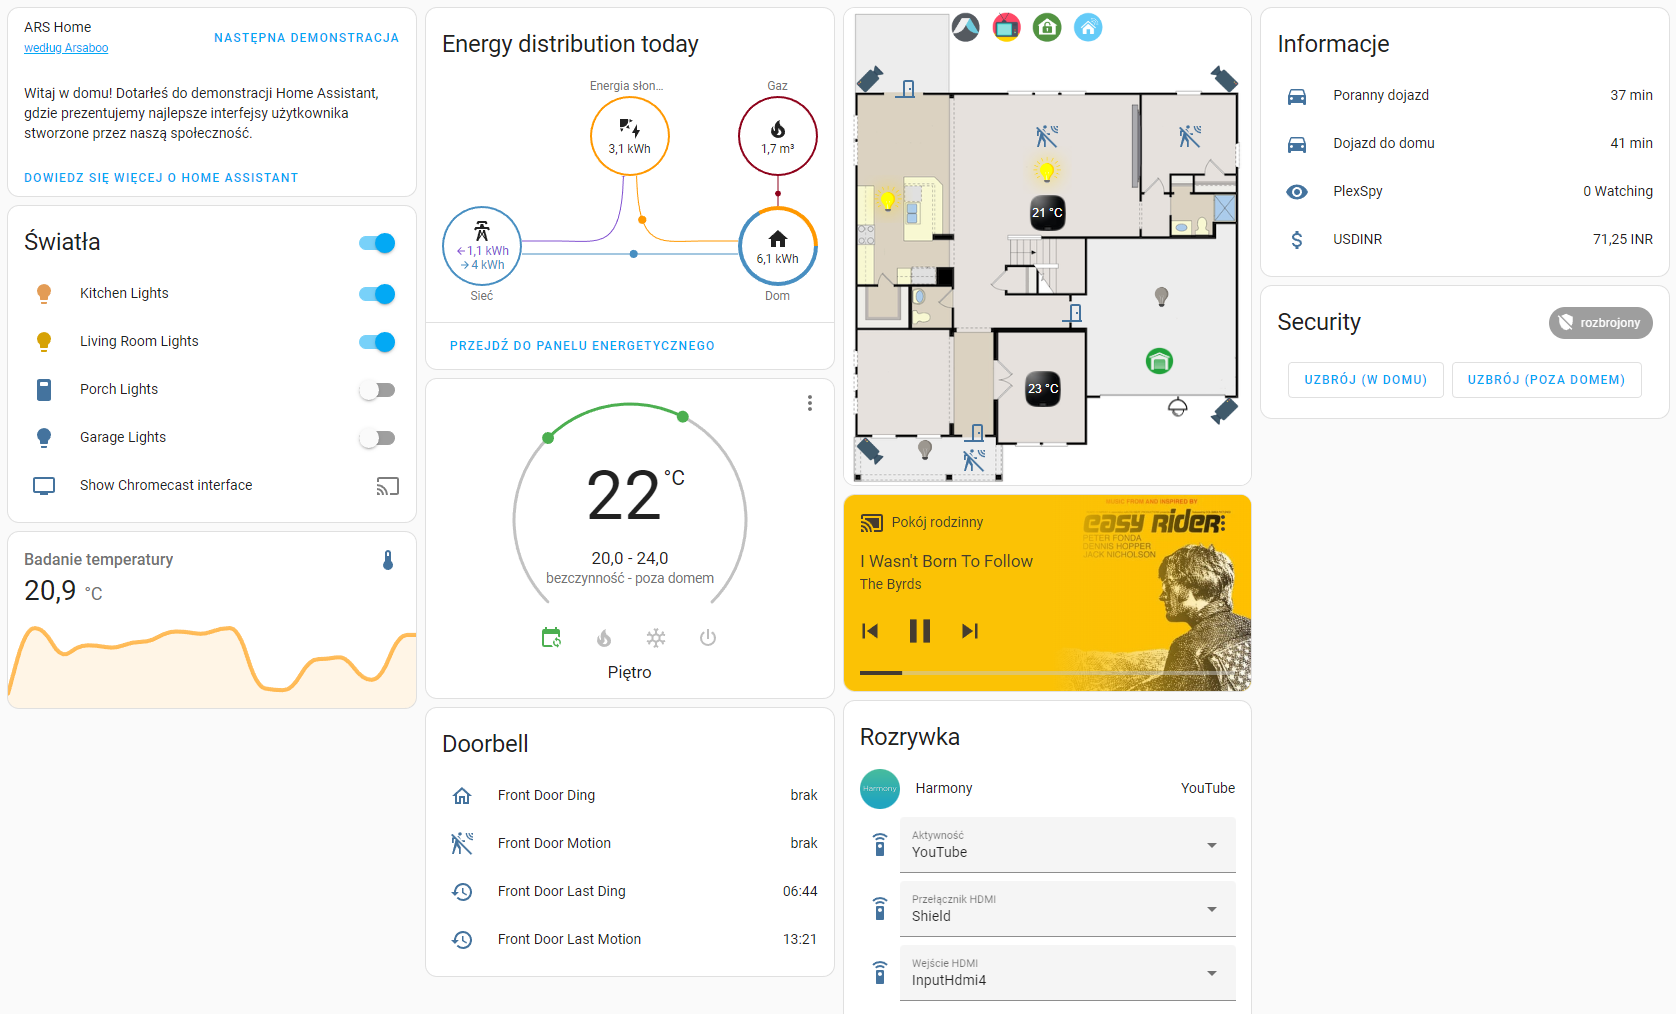
\includegraphics[width=1.00\textwidth]{img/ha_dashboard.png}
    \caption{Przykładowy panel sterowania domem dostarczony przez HomeAssistant} \label{fig:dashboard_example}
\end{figure}

% https://analytics.home-assistant.io/

\subsection{AppDaemon -- AD}
System pozwalający stworzenie modułu samouczącego powinien dawać maksimum możliwości i niezależności, zatem wybrano \textit{AppDaemon}. Jest to środowisko wykonawcze języka programowania Python, w wielowątkowej architekturze piaskownicy, służące do pisania aplikacji automatyzacji dla projektów automatyki domowej (i nie tylko), których wymogiem jest solidna architektura sterowana zdarzeniami. AD zaraz po uruchomieniu jest gotowe do współpracy z systemem \textit{HomeAssistant}, co sprawia, że integracja systemów HA/AD jest bezproblemowa. System pozwala natychmiastowo reagować na zmiany stanów urządzeń znajdujących się w domowym środowisku, poprzez korzystanie z asynchronicznej architektury callback.
% Wybór HA jako systemu nadzorczego ogranicza nam pole wyboru rozwiązań które

\subsection{Python i Tensorflow -- tf}
Wykorzystanie struktury HA/AD ogranicza projekt do wyboru jezyka Python jako przewodniego języka programowania w tym przedsięwzięciu. Taki wybór nie jest jednak ograniczeniem w tym projekcie, ponieważ posiada on bardzo wielką rzeszę fanów tworzących i udoskonalających paczki kodu dodające nowe możliwości w celu powiększenia pola zastosowań tego języka.

Konkretnym jednym zastosowaniem, który w ostatnim czasie budzi wiele uwagi, jest użycie języka Python do celów uczenia maszynowego. Jedną z bibliotek dostarczających rozwiązania związane z tworzeniem, "uczeniem" i eksploatacją modeli różnego rodzaju sieci neuronowych jest paczka \textit{Tensorflow}. Tf implementuje wiele gotowych modeli i algorytmów przyspieszających tworzenie modeli sieci neuronowych. Dodatkowo w celu przyspieszenia procesu liczenia błędu propagacji, biblioteka korzysta z różnego rodzaju akceleratorów obliczeń, w tym kart graficznych.

\subsection{Docker}
Ze względu na wymóg niezależności od platformy na jakiej będzie znajdować się ten system, zdecydowano o wyborze jako jednej z głównych technologii, systemu Docker w celu zapewnienia aplikacjom pracującym w jego środowisku odpowiednich warunków niezależnie od systemu operacyjnego na jakim się znajdują. Dodatkowym powodem, który sprawił że wybrano tę technologię jest gotowe wsparcie systemów HA i AD do pracy w konteneryzowanym środowisku bez dużej ilości konfiguracji. Gotowe obrazy aplikacji znajdują się w sieci, a ich instalacja pod warunkiem posiadania środowiska Docker jest bardzo prosta i szybka.

Dodatkowo narzędzia które dostarcza Docker, pozwalają na tworzenie własnych kontenerów i udostępnianie ich innym co sprawi, że nie będzie to rozwiązanie przygotowywane specjalnie pod konkretne środowisko automatyki.

\subsection{Pozostałe narzędzia i biblioteki}
W celu zarządzania środowiskiem programistycznym, wykorzystano platformę \textit{Pipenv}, która to ułatwia zarządzanie wirtualnymi środowiskami języka Python oraz ułatwia instalację wszystkich bibliotek potrzebnych w danej bazie kodu. Aby wytworzyć gotową paczkę kodu która dalej, która zostanie zainstalowana w AD, wykorzystano narzędzie \textit{setuptools}. Do wszelakich numerycznych obliczeń oraz interfejsu z Tensorflow została wykorzystana biblioteka \textit{numpy}. Automatyzowanie środowiska programistycznego zostało wykonane za pośrednictwem \textit{Makefile}. 

W celu poprawy jakości możliwego w przyszłości rozszerzenia projektu, zdecydowano o skorzystaniu z kilku programistycznych udogodnień. Cała praca podczas tworzenia będzie zapisywana w systemie kontroli wersji \textit{git}, gdzie będzie można cofać lub wprowadzać zmiany w kodzie na różnych gałęziach niezależnie od siebie. Dodatkowo skorzystano z narzędzia \textit{pre-commit}, dzięki któremu przed każdym zapisem konkretnej wersji modułu do systemu kontroli wersji, na kodzie będzie przeprowadzana statyczna analiza oraz pewne porządki mające na celu poprawę jakości pracy nad kodem.


\subsection{Podsumowanie}
Na rysunku (\ref{fig:architektura}) znajduje się zaproponowana architektura wysokopoziomowa środowiska. Urządzenia automatyki znajdujące się w domowym środowisku będą komunikowały się z HomeAssistant w celu aktualizowania swojego stanu, ten będzie przesyłany dalej do AppDaemon, gdzie będzie znajdował się moduł obsługujący wybrane zdarzenia. Korzystając z informacji o zdarzeniu, system będzie przewidywał następną akcję i wykonywał pozostałą przewidzianą w danym epizodzie zmianę stanu. Informację o poleceniu zmiany stanu będzie obsługiwał AD, który to dalej bedzie przesyłał tę informację do HA, który zdecyduje jak z danym urządzeniem się skomunikować i jaką wiadomość wysłać. 

\begin{figure}
    \centering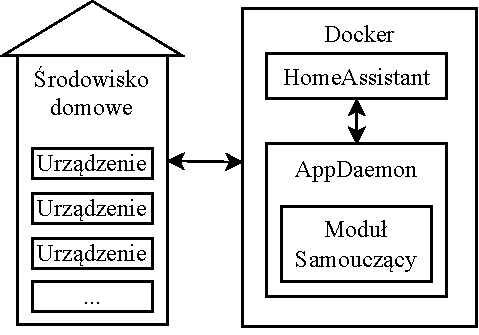
\includegraphics[width=.45\textwidth]{img/architecture.pdf}
    \caption{Proponowane środowisko rozwiązania problemu.} \label{fig:architektura}
\end{figure}

Wewnątrz bloku z modułem samouczącym znajdzie się dopiero kod napisany w języku Python, który będzie reagował na zmiany stanu i w odpowiedni sposób go preparował do przekazania modelowi sieci neuronowych a następnie przekształcany do formy umożliwiającej sterowanie urządzeniami w domu.

\section{Architektura modułu}
Ze względu na wymóg obsługi różnych typów urządzeń oraz źródeł danych, bardzo ważnym aspektem do zaprojektowania jest struktura systemu tłumaczącego dane na takie które, zrozumie biblioteka Tensorflow, zaprojektowanie samych modeli głębokich sieci neuronowych, ale także tłumaczenie wygenerowanej przez model odpowiedzi do takiej, którą zinterpretuje reszta modułu.

\subsection{Dane wejściowe i wyjściowe}
System zarządzania automatyką domową podczas swojej pracy zbiera informacje na temat zmian stanów urządzeń którymi steruje i zapisuje je w lokalnej bazie danych. Nie jest ona jednak dostępna w łatwy sposób dla programisty. AppDaemon w swoim interfejsie programistycznym udostępnia możliwość pobrania historii zmian stanu wybranego urządzenia z ostatniego czasu. Dane przekazane z zapytania do aplikacji są w postaci listy słowników języka Python o strukturze zawartej w listingu (\ref{listing:appdaemon_history}), z której usunięto wszystkie nieważne dla modułu pola. Słownik to pewna struktura danych w której informacja jest zawarta w wartościach dla konkretnego klucza \cite{book:learning_python}.

\begin{listing}
\begin{minted}{python}
[
    {
        "entity_id": "input_boolean.test_switch_1",
        "state": "off",
        "last_changed": "2023-09-11T13:07:52.856406+00:00",
        "last_updated": "2023-09-11T13:07:52.856406+00:00"
    },
    ...
]
\end{minted}
\caption{Historyczne informacje na temat stanu urządzenia pochodzące z systemu AppDaemon.} \label{listing:appdaemon_history}
\end{listing}

Warto zauważyć, że informacja zawarta w polu \verb+state+, ma inne znaczenie w zależności od typu urządzenia czy źródła. W przypadku urządzenia typu przerzutnik stabilny o binarnych pozycjach, dane w kluczach \verb+state+ oraz \verb+last_changed+ wskazuje na czas kiedy zaszła zmiana do jakiego stanu, a w przepadu zwykłego przycisku, wystarcza samo pole ze stanem, ponieważ znajduje się tam czas ostatniej zmiany. Dodatkowo, wartości pola stanu nie ograniczają się do prostych wartości. System HomeAssistant dodaje kilka dodatkowych wirtualnych urządzeń, które zmieniają swój stan raz dziennie, a ich wartość stanu przy każdej zmianie przyjmuje czas, np. następnego wschodu czy zachodu słońca.

W celu zaspokojenia wymagania integracji z wieloma urządzeniami system powinien na podstawie dostarczonej mu informacji o typie urządzenia tłumaczyć ciąg historycznych zmian na dane treningowe do modelu sieci. Aby rozszerzenie tego rozwiązania było możliwe przez użytkownika, proponuje się, aby system korzystał z klas abstrakcyjnych. Pozwoli to na stworzenie bazowego obiektu i określeniu funkcji jakie powinno obsługiwać dane urządzenie w celu współpracy z modułem \cite{book:czysty_kod}. Dodatkowo wymusi to na użytkowniku tworzącym dodatkowe elementy, stworzenie wszystkich wymaganych funkcji, a nie jej pewnej części, co pomoże w redukcji błędów programistycznych.

W celu odpowiedniego przygotowania danych wyjściowych pochodzących z sieci neuronowej, można skorzystać z zaproponowanego wyżej kodu obsługującego dane wejściowe poprzez stworzenie dodatkowych funkcji obsługujących przemiane danych w odwrotnym kierunku. % , które muszą zostać stworzeone do prawidłowego działania systemu.

Proponowana struktura danych na której moduł będzie się opierał to zestaw dwóch macierzy (\ref{eq:opis_stanu}). Pierwsza zawierająca informacje o aktualnym stanie systemu składająca się z $u$ informacji wejściowych nazywana macierzą stanu, druga składająca się z $w$ skalarów opisująca zmiany w stanach nazywana macierzą przejścia. 

\begin{align}
    \begin{split}
        \mathbf{S}_t = \left[s_1, s_2, \dots, s_u\right] \\
        \mathbf{Z}_t = \left[z_1, z_2, \dots, z_w\right]
    \end{split}
    \label{eq:opis_stanu}
\end{align}

% todo: nie mam nigdzie napisane co to epizod, wypadało by tutaj
% &\text{Przykładowo}\ \left[0, 32, 16, 1\right]
% &\text{Przykładowo}\ \left[-1, 0, 0,  1\right]
% Przykładowo zakładając macierz 

Pierwsza z nich opisuje stan środowiska domowego w danym momencie $t$, druga z nich wskazuje na zmianę stanu urządzeń do następnego momentu w czasie $t+1$. Jesteśmy w stanie określić pewną funkcję $G$ w zależności od typów urządzeń i źródeł, która na podstawie aktualnego stanu oraz zmiany w danym momencie, generuje nam następną macierz $\mathbf{S}_{t+1}$ (\ref{eq:opis_przejscia}).

\begin{align}
    G\left(\mathbf{S}_t, \mathbf{Z}_t\right) &= \mathbf{S}_{t+1} \label{eq:opis_przejscia} \\
    \mathbf{Z}_k &= P(\mathbf{S}_k) \label{eq:opis_modelu}
\end{align}

Biorąc powyższe pod uwagę, proponowane rozwiązanie powinno na podstawie macierzy stanu $\mathbf{S}$ w momencie $k$ przewidywać następny zestaw ruchów użytkownika, czyli macierz przejścia $\mathbf{Z}$ dla tego samego momentu w czasie (\ref{eq:opis_modelu}).

\subsection{Architektura głębokich sieci neuronowych} \label{subsec:nn}
Sercem pracy całego modułu są modele matematyczne sieci neuronowych. Ze względu na wymóg minimalnej konfiguracji, ich logiczna konfiguracja, powinna być wybrana tak, aby były w stanie nauczyć się epizodów akcji użytkownika bez zbędnej wielkości i skomplikowania. Dodatkowym powodem ograniczenia skomplikowania takich sieci jest zdecydowane wydłużenie procesu uczenia sieci neuronowych dla tych które, zawierają dużo wag \cite{time_complexity_nn}.

Model sieci neuronowej zawarty w takim module będzie pracował z różnymi typami urządzeń wejściowych gdzie dane będą sformatowane w różny sposób, dodatkowo dane wyjściowe będą musiały być interpretowane przez moduł inaczej, w zależności od celu. Tworzenie dużych i skomplikowanych sieci nie zawsze sprawia, że jest ona w stanie lepiej nauczyć się przekazywanych jej danych ze względu na klątwę wymiarowości \cite{curse_of_dimensionality}.

Biorąc powyższe pod uwagę, proponuje się, aby moduł podczas tworzenia początkowych modeli nie tworzył jednej monolitycznej sieci odpowiedzialnej za wszystkie wejścia i wyjścia, a tworzył tyle sieci, ile jest urządzeń do sterowania. Umożliwi to sieciom lepsze dostosowanie sie do urządzeń i natury ich używania kosztem nieznacznie dłuższego czasu uczenia.

Proponowana struktura takich sieci znajduje się w tabeli (\ref{tab:neural_network}). Pierwsza warstwa w tym modelu będzie zależna od ilości urządzeń i źródeł dodatkowych danych, a ostatnia warstwa będzie zawierała jedno wyjście. Taka struktura, będzie agregowała wszystkie wyjścia do jednej formy dostarczanej reszcie komponentów.

\begin{table}
    \centering\caption{Tabela zawierająca listowanie warstw w pojedynczej sieci neuronowej \label{tab:neural_network}}
    \begin{tabular}{|l|l|l|}
        \hline
        Warstwa     & Aktywacja     & Ilość neuronów    \dnl
        0           & \verb+linear+ & Zależna od ilości urządzeń    \nl
        1           & \verb+ReLU+   & 128               \nl
        2           & \verb+ReLU+   & 64                \nl
        3           & \verb+tanh+   & 1                 \nl
    \end{tabular}
\end{table}

\subsection{Eksport i import sieci}
Aby móc zapisać modele sieci neuronowych, wszystkie części systemu mające z nimi styczność muszą wspierać takie działanie. W szczególności dwoma krytycznymi elementami w przypadku tego modułu samouczącego jest biblioteka Tensorflow oraz tworzony przez nas system konwersji danych. Oba te elementy powinny współpracować ze sobą na tyle dynamicznie, aby różne konfiguracje modeli oraz danych wejściowych były poprawnie obsługiwane.

Biblioteka Tensorflow dostarcza swoje metody na zapis i odczyt modeli do pamięci stałej, ale są one ograniczone z kilku powodów. Jednym z nich jest brak możliwości zapisywania struktury i wag do własnego bufora w pamięci czy swojego deskryptora pliku. Sprawia to, że każda osobna zapisana sieć będzie tworzyła jeden osobny plik na dysku, dodatkowo bez możliwości dołączenia własnych danych. Operowanie na dużej ilości urządzeń obsługiwanych przez moduł będzie generowało jeszcze więcej plików, które mogą zostać uporządkowane do postaci jednego, czytanego raz w fazie rozruchu systemu.

W celu eksportu i importu sieci zostanie zaproponowany teoretycznie autorski sposób serializowania i deserializowania danych \cite{book:serialization_deserialization} w którym wszystkie definicje oraz równie ważne -- wagi wyuczonych sieci neuronowych zostaną zapisane w odpowiednim formacie do pliku archiwum \verb+.zip+. Zapisanie wszystkich potrzebnych informacji do odtworzenia całej struktury w jednym pliku ułatwi przenoszenie użytkownikowi systemu między komputerami, ale także zniechęci go od ewentualnego ręcznego zmieniania wartości wag w systemie, poprzez zaciemnienie widocznej struktury.

Proponowana architektura plików wewnątrz archiwum dla każdej z sieci osobno będzie składała się z:
\begin{enumerate}
    \item Surowej deklaracji modelu, w której znajdzie się dokładny opis kształtu i wymiarów każdej z warstw potrzebnej do dokładnego jej odtworzenia.
    \item Pliku z zapisanymi wagami każdej warstwy w sieci.
    \item Pliku z informacjami pośrednimi, które nie są krytyczne do działania systemu.
\end{enumerate}

Dodatkowo w celu określenia czy nie doszło do zmiany dostępnych dla systemu urządzeń oraz w celu zapisania innych informacji ogólnych o wszystkich dostępnych w modelu sieciach będzie potrzebny jeden dodatkowy plik znajdujący się katalogu głównym archiwum.

\subsection{Podsumowanie}
Na rysunku (\ref{fig:architektura_modułu}) znajduje się proponowana struktura całego modułu samouczącego. Dane o stanie i zmianach będą przechodziły strumieniem wgłąb systemu. Dalej po obliczonej na podstawie stanu systemu predykcji, system będzie sterował urządzeniami w środowisku domowym.

\begin{figure}
    \centering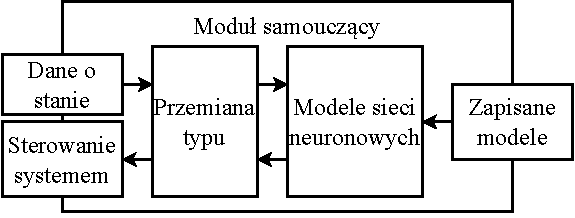
\includegraphics[width=.55\textwidth]{img/architecture_module.pdf}
    \caption{Proponowana struktura działania modułu.} \label{fig:architektura_modułu}
\end{figure}

% \subsection{Sterowanie systemem}

% Sprawia to, że gdy użytkownik posiada istniejącą i skonfigurowaną instalację HomeAssistant z której korzysta, dodanie tego modułu powinno od razu zacząć działać.
% Dane wejściowe obsługiwane przez system przekazywane do biblioteki uczenia maszynowego powinny posiadać swoją pewną strukturę, umożliwiającą Tensorflow pracę.
\chapter{Implementacja}

\section{Dane wejściowe}
Krok przemiany danych wejściowych do wykorzystania w module został podzielony na dwa osobne etapy. Jeden z tych etapów, nazywany krokiem interpretacji różni się w zależności od źródła skąd pochodzą dane. W zależności od tego, czy system korzysta z danych historycznych w procesie uczenia, czy korzysta z danych aktualnych w celu predykcji inaczej przechodzą proces interpretacji. Drugim etapem jest etap transformacji i wygląda on tak samo dla każdego źródła niezależnie od typu.

\subsection{Interpretacja historyczna}
W przypadku źródła danych historycznych, system musi rozpoznawać epizody działań domowników w celu ich nauki. W tym celu, aby wygenerować zbiór danych uczących, przegląda się posortowaną listę wydarzeń w czasie, celem określenia epizodów akcji. Począwszy od pierwszego wydarzenia w dostępnej dla systemu historii, przegląda się ją w poszukiwaniu ciągu akcji o łącznym czasie nie większym niż pewien z góry określony parametr nazwany \verb+EPISODE_DELTA+ od momentu wystąpienia pierwszej akcji w epizodzie. Ta wartość została wprowadzona w celu sprawdzenia czy zmiana stanu w epizodzie się nie przedawniła. W przypadku gdy jedno urządzenie zmienia swój stan kilkukrotnie w przeciągu jednego epizodu, brana jest tylko pod uwagę policzona zmiana i stan względem poprzedniego, przed liczonym epizodem. W tabeli (\ref{tab:znaleziony_epizod}) został zaznaczony znaleziony dla przykładowej historii epizod. Kolorem został zaznaczony znaleziony przez algorytm epizod akcji. 

Warto zauważyć, że wybrana długość tego parametru będzie mocno wpływała na liczność i wielkość epizodów. Wybranie zbyt krótkiego czasu epizodu będzie rozdzielać powiązane ze sobą czynności ale będzie rozróżniała zmiany stanu tego samego urządzenia w czasie, a wybranie zbyt długiego czasu będzie łączyło kilka niezależnych akcji ze sobą, możliwie je ze sobą niwelując. Sprawia to, że wybranie optymalnej długości epizodu jest bardzo ważne aby system mógł dostosować się do użytkownika.

\begin{table}
    \centering\caption{Tabela przedstawiająca działanie algorytmu szukania epizodów. \label{tab:znaleziony_epizod}}
    \begin{tabular}{|l|l|l|}
        \hline
        Urządzenie              & Stan       & Czas     \dnl
        \dots                   & \dots      & \dots    \nl
        \verb+światło kuchnia+  & \verb+on+  & 16:52:48 \nl 
        \rowcolor{lightgray}
        \verb+światło kuchnia+  & \verb+off+ & 17:32:12 \nl 
        \rowcolor{lightgray}
        \verb+klimatyzacja+     & \verb+17+  & 17:33:00 \nl 
        \rowcolor{lightgray}
        \verb+światło salon+    & \verb+on+  & 17:33:10 \nl
        \rowcolor{lightgray}
        \verb+telewizor salon+  & \verb+on+  & 17:33:15 \nl
        \verb+światło balkon+   & \verb+on+  & 19:32:42 \nl
        \dots                   & \dots      & \dots    \nl
    \end{tabular}
\end{table}

Do określenia działania, dla każdego innego typu urządzeń z osobna, skorzystano z abstrakcyjnej klasy \verb+DeviceHistoryGeneric+, opisujących strukturę funkcji jakie powinna dana klasa implementować w celu poprawnego działania. Abstrakcyjna funkcja na podstawie stanu urządzenia w momencie $t$, stanu urządzenia w momencie $k$ oraz czasu do którego dany epizod powinien się skończyć, zwraca w postaci rzeczywistej liczby, stan oraz przejście stanu dla danego epizodu w czasie. Pseudokod takiej funkcji został zawarty w listingu (\ref{listing:pseudo_get_past_state}). Warto zauważyć, że gdy nie ma poprzedniego stanu, tj. historia nie sięga na tyle wstecz, to kod musi obsługiwać wykrywanie obu wartości. W przypadku interpretacji prostych urządzeń, nie jest to problemem, ponieważ jesteśmy w stanie wydedukować przejście stanu i aktualny stan na podstawie informacji pochodzącej z systemu, tak w przypadku gdy tej możliwości nie ma, pojedynczy błędny wynik powinien być zdecydowaną mniejszością po interpretacji reszty historii.

% todo: zapytać o ten pseudokod
\begin{listing}
\begin{minted}[mathescape]{python}
def get_past_state(aktualny, poprzedni, do_momentu):
    wartość_stanu = 1.0 jeśli aktualny = "on" wpw 0.0
    wartość_przejścia = 0.0
    # Czy mamy historię na temat poprzedniego?
    jeśli poprzedni nie istnieje:
        # zakładamy, że zmiana stanu odbyła się dawno w historii
        return wartość_stanu, wartość_przejścia
    
    # Czy zmiana się nie przedawniła?
    jeśli poprzedni.czas_zmiany < do_momentu:
        wartość_przejścia = 1.0 jeśli aktualny = "on" wpw -1.0

    return wartość_stanu, wartość_przejścia
\end{minted}
\caption{Pseudokod funkcji interpretującej stany ze źródła historycznego dla typu urządzenia przełącznika astabilnego on/off.} \label{listing:pseudo_get_past_state}
\end{listing}

% Zebrane w ten sposób dane, zbierane są jako listy słowników języka Python w celu łatwiejszego 

\subsection{Interpretacja bieżąca} \label{subsec:interpretacja}
Bieżąca interpretacja akcji użytkownika wygląda bardzo podobnie do analizy historycznej. Informacja o bieżącym stanie całego systemu przechowywana jest przez moduł w pamięci. Podczas pracy systemu, mamy pewność, że system AppDaemon zgłosi zmianę stanu tylko jednego urządzenia za każdym uruchomieniem naszej asynchronicznej funkcji. Wiemy zatem, że musimy tylko obsłużyć zmianę stanu jednego urządzenia i zapisać jego stan do pamięci. Informacja o tym, jakie urządzenie zmieniło się do jakiego stanu będzie potrzebna w procesie predykcji, które będzie opisane w późniejszym etapie. Korzystając z tej samej klasy dla typu urządzenia co w przypadku interpretacji historycznej w podobny sposób określamy stan i przejście stanu urządzenia. W tym wypadku ze względu na pewność, że dane urządzenie zmieniło swój stan dokładnie w momencie uruchomienia danej funkcji, obliczanie stanu i przejścia jest zdecydowanie prostsze ponieważ, nie trzeba rozważać przedawnienia się zmiany.

\subsection{Transformacja} \label{subsec:transformacja}
Po prawidłowej ekstrakcji zmian stanu, przed przekazaniem ich do sieci neuronowych dane są dodatkowo przekształcane. W przypadku prostych urządzeń typu przełączniki astabilne, ten proces nie wprowadza do danych żadnej zmiany. W przypadku bardziej skomplikowanych typów danych, takich jak zmienne temporalne wskazujące na np. dzień tygodnia, czy porę dnia, przeprowadzane są pewne dodatkowe operacje rozkładające jedną konkretną informację na kilka różnych wartości, które lepiej będzie sieciom neuronowym powiązać ze akcjami. W celu możliwości wprowadzenia rozszerzalności tutaj ponownie wykorzystano podejście obiektowe i skorzystano z klasy abstrakcyjnej. Zaproponowana klasa abstrakcyjna \verb+Convertable+ opisuje dwie funkcje, które dany konwerter danych musi zaimplementować. Jedna z nich opisuje przejście danych do wersji akceptowalnej przez sieci neuronowe, druga tłumaczy dane wygenerowane przez sieć neuronową do formy obsługiwanej przez resztę systemu. Jednym specjalnym przypadkiem takiego konwertowania danych gdzie potrzebna jest zaimplementowana jedna z obu funkcji, jest przekazywanie zmiennych temporalnych do sieci.

W celu przekazania do sieci jak największej ilości rzeczywiście użytecznych informacji o porze dnia, tak aby była ona w stanie w swojej strukturze zapisać nawyki użytkownika, informacja o czasie jest podzielona. Podział jednej zmiennej czasowej odbywa się poprzez podzielenie jej na 24 różne informacje, gdzie każda z nich wskazuje na pewną wartość zależną od odległości indeksu danej zmiennej od godziny wydarzenia epizodu. Dokładniej, jest to wartość funkcji Gaussa dla wartości zależnej od indeksu, z parametrem $\mu$ ustawionym na moment w ciągu dnia podczas którego wydarzył się ten epizod.

Ważnym parametrem w przypadku funkcji Gaussa poza parametrem $\mu$, jest parametr opisujący szerokość dzwona. W zastosowaniach statystycznych nazywany odchyleniem standardowym $\sigma$. W przypadku takiego zastosowania obliczania wartości funkcji na podstawie czasu, szerokość mówi nam o tym, jak bardzo akcje występujące o konkretnej porze w ciągu dnia mogą być proponowane o innych podobnych godzinach. Ustawienie tego parametru zbyt szeroko, spowoduje że system będzie rozpoznawał wykonywanie konkretnych akcji o bardzo szczegółowych godzinach w ciągu dnia, ustawienie tego za szeroko, będzie proponowało wykonywanie akcji nieadekwatnych do konkretnej pory dnia. Na obrazie (\ref{fig:time_param}) znajduje się przykładowy zarys wartości funkcji dla kilku konkretnych pór dnia, razem z zaznaczonymi dokładnymi przebiegami krzywizny dzwonowej. Każda z zaznaczonych godzin posiada inny parametr $\sigma$ w celu pokazania wpływu tego parametru na policzone wartości.

\begin{figure}
    \centering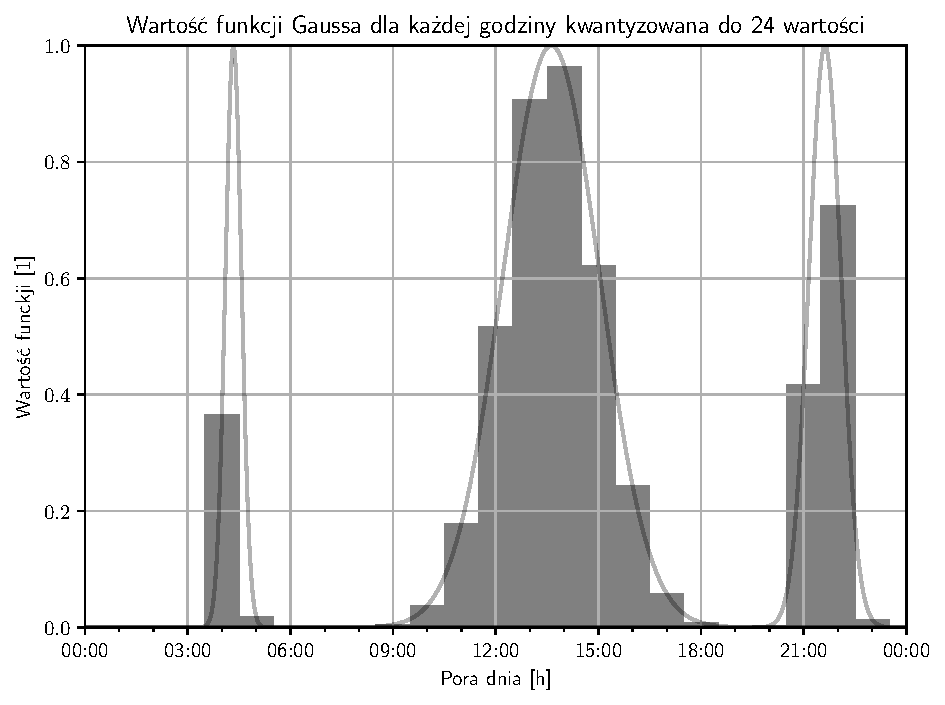
\includegraphics[width=1.00\textwidth]{img/time_param.pdf}
    \caption{Policzone wartości funkcji Gaussa wskazującej czas dla godziny 4:20:02, 13:37:21, 21:37:21.} \label{fig:time_param}
\end{figure}


\section{Sieci neuronowe}
Ze względu na wymóg osobnego przetwarzania wielu źródeł różnego typu w systemie, gdzie część z nich może kolejno zostać jeszcze podzielona na dalsze drobniejsze informacje, całość systemu została umieszczona w obiekt będący menedżerem. Głównym zadaniem menedżera jest agregowanie do jednego obiektu wielu konwerterów i agentów. Agent w tym systemie, to obiekt z pewnymi z góry określonymi funkcjami opakowujący modele matematyczne dostarczone przez bibliotekę Tensorflow wykorzystywany do schowania za warstwą abstrakcji, detali implementacji \cite{book:programming_abstraction}, \cite{book:czysty_kod}. Takie wykorzystania menedżerów i obiektów agregujących przydaje się w przypadku tworzenia systemów dynamicznych polegających na wczytywaniu i zapisywaniu obiektów do pamięci stałej. W przypadku tego modułu samouczącego, daje to osobie rozszerzającej, możliwości wykorzystania innych struktur niż wcześniej określono (\ref{tab:neural_network}) lub nawet wykorzystanie kompletnie innych metod predykcji w celu osiągnięcia danego celu.

\subsection{Dynamiczne tworzenie}
Jedną bardzo wygodną możliwością udostępnianą przez bibliotekę Tensorflow dla modeli sieci neuronowych są nazwane wyjścia oraz wejścia dla sieci. Pozwala to na dynamiczne tworzenie i eksploatację modeli bez żadnego bardzo skomplikowanego systemu przetwarzającego nazwę wejść na globalną pozycję w macierzy wejściowej. System w celu stworzenia modelu sieci neuronowej wykorzystuje obiekt \verb+Model+ udostępniany przez bibliotekę wykonawczą Tensorflow -- Keras. Do stworzenia modelu sieci neuronowej, korzystamy z informacji o nazwach wejść oraz nazwach wyjść. System podczas tworzenia nowej sieci, tworzy listę warstw typu \verb+Input+ i każdej z nich przypisuje nazwę kolejnego wejścia do sieci, następnie każda z tych warstw, o kształcie \verb+(wielkość próbki, 1)+, jest do siebie dodawana wzdłuż drugiego wymiaru za pomocą warstwy typu \verb+Concatenate+. Powstała warstwa ma kształt \verb+(wielkość próbki, ilość wejść)+. W tym momencie kolejne warstwy dodaje się tak samo jak w przypadku zwykłego modelu funkcyjnego biblioteki Tensorflow i następuje zgodnie z listą warstw podaną we wcześniejszym rozdziale (\ref{tab:neural_network}). Ostatnia warstwa, ta wyjściowa, tak jak w przypadku warstw wejściowych generowana jest z listy nazw wyjść. Dynamiczne tworzenie wyjść, razem z modelem modularnej transformacji, opisanej wcześniej, daje bardzo potężne narzędzie do sterowania domem.

\subsection{Serializowanie i deserializowanie}
Zapis oraz import danych w systemach komputerowych z formy istniejącej w pamięci do formatu, którą można zapisać na dysk jest bardzo dużym zagadnieniem samym w sobie. W przypadku języka Python jest bardzo dużo możliwości godnych tego zadania. Istnieje wbudowana biblioteka taka jak Pickle, która zapisuje wprost bit po bicie zawartość pamięci programu do pliku na dysku, ale zapisuje bardzo dużo redundantnych informacji nad którymi nie mamy kontroli. Istnieją rozwiązania które są czytelne dla ludzi, ale osiągają mniejszą efektywność zapisu danych, takie jak XML \cite{book:xml_handbook} czy JSON \cite{book:json_for_begginers}. 

W wypadku zapisu i odczytu modeli matematycznych potrzebna jest obsługa trzech różnych informacji, które zostały wymienione wcześniej (\ref{subsec:nn}). Opis logicznej struktury sieci, składa się z informacji o każdej z warstw. Każda z warstw zawiera informacje o jej wielkości, typie, rodzaju aktywacji, nazwach oraz informacji z jakimi warstwami sąsiaduje. Dostarczana przez Tensorflow metoda dla obiektu modelu zwraca wszystkie te informacje w postaci słownika, zawierającego tekst, listy oraz kolejne warstwy słowników. Klasa odpowiedzialna za model implementuje konstruktor \cite{book:czysty_kod}, który korzystając z informacji zawartych w opisanym słowniku odtwarza dokładną strukturę modelu. Sytuacja wygląda bardzo podobnie dla wag w modelu. Każda warstwa udostępnia funkcję zwracającą listę wszystkich ważnych dla danego typu warstwy parametrów, a druga w obiekcie modelu, przyjmuje listę tych parametrów w celu odtworzenia wag.

W celu implementacji zapisywania i odczytu danych z dysku skorzystano z wbudowanej w Python biblioteki obsługującej pliki \verb+.zip+ oraz z metody serializacji JSON. Do obsługi procesu zapisu i odczytu stworzono klasę \verb+ModelSerializer+, implementującą metody potrzebne do skorzystania z danego obiektu jako menedżera kontekstu języka Python \cite{book:learning_python}. Taki sposób implementacji zapewni, że wszystkie wymagane operacje na pliku i buforach w pamięci zostaną wykonane bez ingerencji użytkownika, co pozwoli na uniknięcie błędów. Stworzony obiekt dostarcza dwie główne metody. Jedna z nich służąca do odczytu i odtworzenia całej struktury menedżerów do takiej wykorzystanej przez moduł oraz drugiej wykorzystywanej do zapisu całego menedżera do pamięci stałej, które działają analogicznie w odwrotnym kierunku.

Pewną emergentną zaletą takiego połączenia serializowania za pomocą JSON wewnątrz kompresowalnego archiwum plików jest zmniejszenie miejsca które zajmują wszystkie modele na dysku, o nawet 57\%. Opis wytworzonego w ten sposób archiwum znajduje się w listingu (\ref{listing:zipinfo}).

\begin{listing}
\begin{minted}{text}
Zip file size: 698977 bytes, number of entries: 19
?rw-------  2.0 unx     8626 b- 23-Nov-22 10:47 kuchnia/declaration.json
?rw-------  2.0 unx   264887 b- 23-Nov-22 10:47 kuchnia/weights.json
?rw-------  2.0 unx       59 b- 23-Nov-22 10:47 kuchnia/meta/info.json
?rw-------  2.0 unx     8640 b- 23-Nov-22 10:47 ekspres/declaration.json
?rw-------  2.0 unx   265319 b- 23-Nov-22 10:47 ekspres/weights.json
?rw-------  2.0 unx       59 b- 23-Nov-22 10:47 ekspres/meta/info.json
?rw-------  2.0 unx     8646 b- 23-Nov-22 10:47 salon/declaration.json
?rw-------  2.0 unx   265341 b- 23-Nov-22 10:47 salon/weights.json
?rw-------  2.0 unx       59 b- 23-Nov-22 10:47 salon/meta/info.json
?rw-------  2.0 unx     8648 b- 23-Nov-22 10:47 telewizor/declaration.json
?rw-------  2.0 unx   265556 b- 23-Nov-22 10:47 telewizor/weights.json
?rw-------  2.0 unx       59 b- 23-Nov-22 10:47 telewizor/meta/info.json
?rw-------  2.0 unx     8656 b- 23-Nov-22 10:47 balkon/declaration.json
?rw-------  2.0 unx   265197 b- 23-Nov-22 10:47 balkon/weights.json
?rw-------  2.0 unx       59 b- 23-Nov-22 10:47 balkon/meta/info.json
?rw-------  2.0 unx     8658 b- 23-Nov-22 10:47 sypialnia/declaration.json
?rw-------  2.0 unx   265469 b- 23-Nov-22 10:47 sypialnia/weights.json
?rw-------  2.0 unx       59 b- 23-Nov-22 10:47 sypialnia/meta/info.json
?rw-------  2.0 unx      273 b- 23-Nov-22 10:47 info.json
19 files, 1644270 bytes uncompressed, 696557 bytes compressed:  57.6%
\end{minted}
\caption{Listowanie plików wewnątrz archiwum zawierajacego przykładowe modele sieci pochodzące z programu zipinfo.} \label{listing:zipinfo}
\end{listing}

\section{Sterowanie systemem}
Gdy dane o stanie z dołączonymi innymi informacjami temporalnymi przejdą przez cały system i jest zwracana predykcja, system musi podjąć decyzję czy to co aktualnie użytkownik tych urządzeń wykonuje, jest zgodne z tym co system przewiduje. Jak wcześniej zostało opisane, system stara się przewidzieć następną zmianę stanu na podstawie przekazanych do modelu wartości o aktualnym stanie. Aby system był jak najbardziej wygodny dla użytkownika, zdecydowano na dopełnianie akcji użytkownika zamiast wykonywanie zadań autonomicznie. Sprawia to, że proces wyboru kiedy system powinien dokończyć daną akcję staje się bardzo skomplikowany.

W celu wykonywania tylko tych akcji, które są w danym momencie zgodne z zamiarem użytkownika porównywane są predykcje systemu z aktualną zmianą, na którą moduł reaguje. Dane wejściowe policzone z interpretacji bieżącej (\ref{subsec:interpretacja}) porównywane są z tym co przewiduje system. Jeśli zamiar użytkownika jest wspólny z tym co system chce wykonać, system podejmuje decyzję o dokończeniu przewidzianego epizodu akcji. Porównanie zamiaru jest trywialne i porównuje obliczone aktualne przejście stanu dla danego urządzenia oraz to, które powstało z predykcji. Korzystając z informacji o aktualnym stanie, przewidzianej zmiany, generowane są zapytania do systemu mające na celu sprowadzenie systemu do nowego stanu.

\section{Formatowanie danych uczących} \label{sec:dane_uczace}
Uczenie sieci neuronowych z danych pochodzących z historii HomeAssistant często samo w sobie jest niewystarczające. Sieci mimo tego, że uczone są na dużej ilości danych temporalnych poza samymi stanami systemu, nie są w stanie nauczyć się konkretnych epizodów. W tym celu, zaproponowano generowanie dodatkowych danych uczących na podstawie wygenerowanych informacji o przejściach, aby poprawić celność systemu.

Algorytm generowania danych tworzy dodatkowe informacje wejściowe zawierające brak zmiany stanu dla konkretnego stanu systemu o innej porze dnia niż wtedy kiedy dany epizod jest wykonywany. W tym celu funkcja tworzy dwa słowniki, jeden dla którego wartościami są listy zawierające czas pewnego wydarzenia, druga dla której wartości to zbiory zmiany stanów. W obu tych słownikach, kluczami są stany dla którego rozpatrywany jest czas czy zmiana. Dalej, dla każdego czasu kiedy dane zdarzenie sie wydarzyło, czyli dla elementow w pierwszym z obu słowników, generowany jest estymator jądrowy danego wydarzenia. W tym celu wykorzystano sumę rozkładów normalnych. Następnie wygenerowany estymator jest odwracany i progowany. Wszystkie wartości powyżej lub poniżej pewnego przedziału są spłaszczane do wartości brzegowych, a następnie przekształcane i skalowane tak, aby suma pola pod wykresem wynosiła 1, a najmniejszą wartością było 0. Proces ten został zobrazowany na obrazie (\ref{fig:transform}). Korzystając z tak wygenerowanego estymatora znormalizowanego i funkcji losującej wartość z przedziału pod warunkiem macierzy prawdopodobieństw, dostarczonej przez numpy, generowany jest zestaw zerowych przejść z czasem pochodzącym z tego rozkładu, a następnie dołączany do listy danych do uczenia. Ten proces ma na celu stworzenie listy dodatkowych danych bez żadnej zmiany dla konkretnego stanu o innej porze w ciągu dnia, tak aby sieci neuronowe powiązały konkretny stan w ciągu dnia z konkretną porą dla danej odpowiedzi. Tak stworzona lista dla konkretnych stanów jest bardzo rzadka -- posiada same zera w przejściach stanów -- co może negatywnie wpłynąć na wynik uczenia sieci neuronowych. W tym celu, aby zrównoważyć stosunek ilości pustych akcji do tych rzeczywistych, do listy danych uczących dodawane są kolejne dane. Dane te losowane są z drugiego słownika dla konkretnie obsługiwanego stanu systemu i dodawane do danych uczących, czyli dopisywane są kopie danego rzeczywistego wydarzenia.

\begin{figure}
    \centering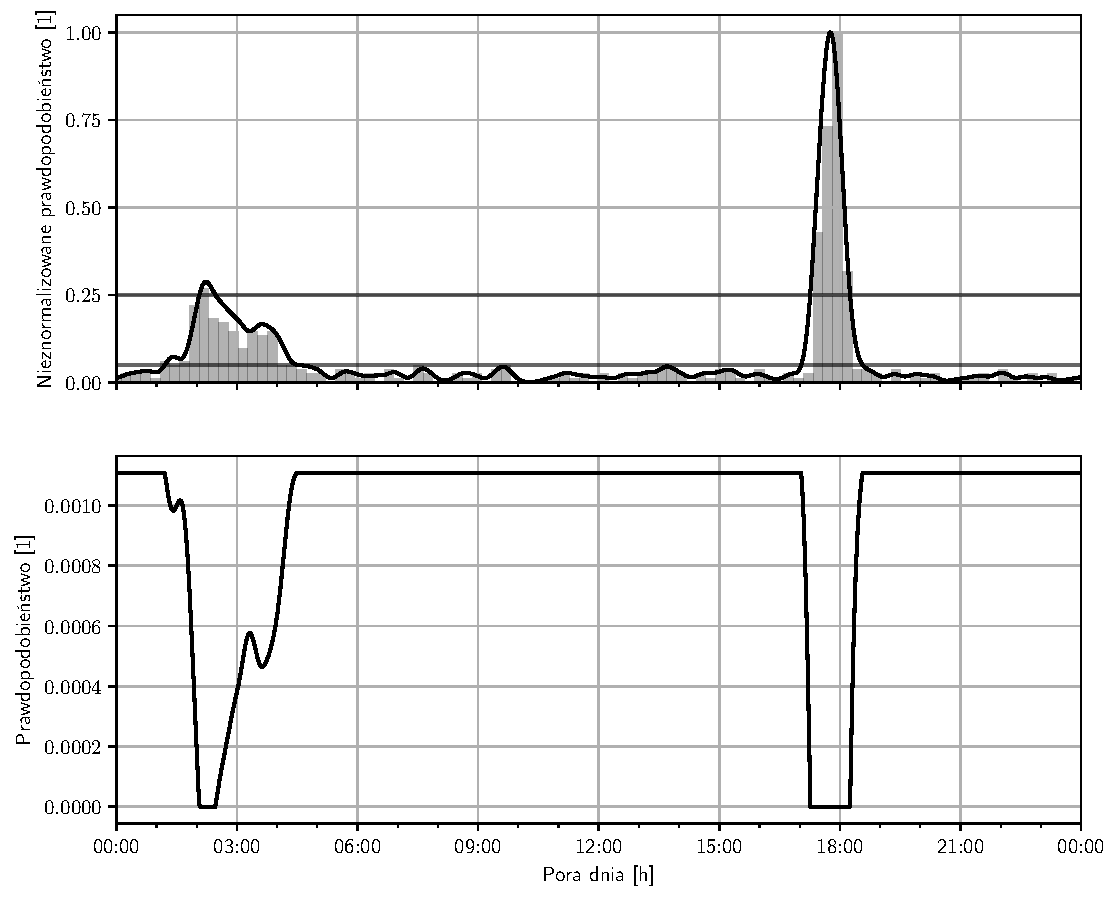
\includegraphics[width=1.00\textwidth]{img/transformation.pdf}
    \caption{Wizualizacja wygenerowanego estymatora jądrowego bez progowania oraz przebieg gotowej funkcji gęstości prawdopodobieństwa.} \label{fig:transform}
\end{figure}

\section{Napotkane problemy}
Ta sekcja ma na celu opisanie zaistniałych problemów podczas implementowania modułu. Są to trudności związane z przewidzeniem jak zachowywać się będzie gotowy system, bez żadnej istniejącej implementacji ani prototypu, ale także, związane ze zwykłą naturą programistyczną.

\subsection{Reprezentacja czasu} \label{subsec:reprezentacja_czasu}
Reprezentacja czasu w modelach uczenia maszynowego jest bardzo ważna. Wysoka i mała rzadkość danych, sprawia, że modele potrzebują bardzo dużo obserwacji aby rzeczywiście były w stanie generować predykcje zgodne z prawdą \cite{curse_of_dimensionality}. Podczas implementacji modułu, początkowo wszystkie dane temporalne, reprezentowane były jako kosinusoida znormalizowanej pory dnia. Wykorzystanie funkcji trygonometrycznej było uwarunkowane jej okresowością i spokojnym przebiegiem przez całą rozpatrywaną domenę. Podczas testów prototypu, bez dodatkowej funkcji tworzącej nowe dane uczące (\ref{sec:dane_uczace}), modele mimo testów z różnymi parametrami nie były w stanie dopasować się do obserwacji. Zdecydowano wówczas o rozbiciu danych temporalnych do zdecydowanie większej i rzadszej formy, zainspirowanej metodami radialnych funkcji bazowych, opisanej w (\ref{subsec:transformacja}). Testy prototypu przynosiły zdecydowanie lepsze wyniki, ale wciąż nie były one wystarczająco zadowalające. Kolejnym krokiem walki który podjęto, było stworzenie wyżej opisanej funkcji generującej sztuczne dane. Dopiero od tego momentu, sieć uczyła się obserwacji w dostatecznym stopniu. Po wstępnych badaniach, okazało się, że poprzednio stworzone rozwiązanie korzystające z funkcji trygonometrycznej i w dalszej iteracji, złożenie sinusoidy i kosinusoidy, w połączeniu z funkcją również dają, zadowalające wyniki. Zdecydowano wtem, o zostawieniu części kodu odpowiedzialnego za pozostały sposób transformacji danych, jako możliwej alternatywy dla użytkownika.

\subsection{Obraz Docker -- AppDaemon}
W celu minimalizacji reimplementacji często używanych i powtarzanych funkcji w językach programowania korzysta się ze standardowych bibliotek, które zapewniają szkielet podstawowych funkcjonalności programowania \cite{book:cstdl}. Pomaga to uniknięcia części błędów i zmniejszenia wielkości powstałego oprogramowania. Każda inna rodzina systemów operacyjnych opiera swoją strukturę na innej bibliotece, które zapewniają w praktyce taką samą funkcjonalność inną implementacją i konwencją, zatem programy nie są kompatybilne między rodzinami systemów operacyjnych, a czasami nawet różnymi dystrybucjami tego samego systemu operacyjnego. Przykładem takiego oprogramowania które nie jest kompatybilne między dystrybucjami tej samej rodziny systemów jest Tensorflow, który jest dostępny w gotowej do zainstalowania wersji między innymi dla systemów wspierających glibc. W celu stworzenia modułu samouczącego, należało połączyć ze sobą obraz AppDaemon wraz z Tensorflow, które w oryginalnych konfiguracjach korzystają z zupełnie innych bibliotek standardowych języka C \cite{page:alpine_linux} \cite{page:ad_dockerfile}. W celu rozwiązania tego problemu, stworzono własny obraz modułu AppDaemon, który powstał na bazie systemu wspierającego glibc. Podczas tworzenia instalowana jest biblioteka Tensorflow oraz opisywany w tej pracy moduł samouczący.

% https://www.alpinelinux.org/about/

% Stworzony, gotowy obraz w internecie modułu AppDaemon bazuje na dystrybucji Linux'a nazywanej Alpine Linux, która opiera się na implementacji musl libc \cite{page:alpine_linux}.
% Gotowe, skompilowane wersje tego oprogramowania są dostępne do pobrania dla systemów korzystających z glibc jako biblioteki standardowej języka C.

% wykorzystanie warstw abstrakcji jest lepsze ...

% !TEX encoding = UTF-8 Unicode 

\chapter*{Podsumowanie}
\section*{Zrealizowana praca}
W ramach tej pracy, przeanalizowano i omówiono zagadnienie związane z automatyką domową. Przejrzano i skategoryzowano istniejące rozwiązania problemu pracy zawarte w literaturze. Każde z podejść zostało poddane analizie w celu rozpoznania mocnych i słabych stron rozwiązania. W dalszej części zagłębiono się w problem zastosowań urządzeń IoT do celów automatyki. Na podstawie literatury i istniejących rozwiązań stworzono zakres wymagań jakie powinien spełniać działający system w celu wspierania użytkownika w codziennych czynnościach domowych. Stworzone wymogi -- funkcjonalne i niefunkcjonalne -- pomogły w określeniu technologii oraz całego środowiska aplikacji w którym stworzony moduł pracuje. Wykorzystanie konkretnych aplikacji, modułów i bibliotek ukształtowało architekturę samego modułu.

\section*{Cel pracy}
Cel prazy został osiągnięty.


% Bibliography
\bibliographystyle{dyplom}
\bibliography{bibliography}

% Lists of figures, listings, tables
\listoffigures
\listoflistings
\listoftables

% Appendices - comment out if not applicable
% \appendixpage
% \appendix
% \chapter{Dodatek 1}\label{app1}

\lipsum[20]

\end{document}
